\documentclass[14pt]{beamer}
\usepackage{hyperref}
\usepackage{ulem}
\usepackage[T1]{fontenc}
\usetheme{Madrid}

% macro for double dash
\newcommand{\dd}{{\texttt{-{}-}}}

%% Enable license helpers
\graphicspath{{../cc_beamer/}}
%%%%%%%%%%%%%%%%%%%%%%%%%%%%%%%%%%%%%%%%%%%%%%%%%%%%%%%%%%%%%%%%
%% ccBeamer 0.1, 2007-07-02                                   %%
%% Written by Sebastian Pipping <webmaster@hartwork.org>      %%
%% ---------------------------------------------------------- %%
%% Licensed under Creative Commons Attribution-ShareAlike 3.0 %%
%% http://creativecommons.org/licenses/by-sa/3.0/             %%
%%%%%%%%%%%%%%%%%%%%%%%%%%%%%%%%%%%%%%%%%%%%%%%%%%%%%%%%%%%%%%%%


%% Images
\newcommand{\CcImageBy}[1]{%
	
\includegraphics[scale=#1]{creative_commons/cc_by_30.pdf}%
}
\newcommand{\CcImageCc}[1]{%
	
\includegraphics[scale=#1]{creative_commons/cc_cc_30.pdf}%
}
\newcommand{\CcImageDevNations}[1]{%
	
\includegraphics[scale=#1]{creative_commons/cc_dev_nations_30.pdf}%
}
\newcommand{\CcImageNc}[1]{%
	
\includegraphics[scale=#1]{creative_commons/cc_nc_30.pdf}%
}
\newcommand{\CcImageNd}[1]{%
	
\includegraphics[scale=#1]{creative_commons/cc_nd_30.pdf}%
}
\newcommand{\CcImagePd}[1]{%
	
\includegraphics[scale=#1]{creative_commons/cc_pd_30.pdf}%
}
\newcommand{\CcImageSa}[1]{%
	
\includegraphics[scale=#1]{creative_commons/cc_sa_30.pdf}%
}
\newcommand{\CcImageSampling}[1]{%
	
\includegraphics[scale=#1]{creative_commons/cc_sampling_30.pdf}%
}
\newcommand{\CcImageSamplingPlus}[1]{%
	
\includegraphics[scale=#1]{creative_commons/cc_sampling_plus_30.pdf}%
}


%% Groups
\newcommand{\CcGroupBy}[1]{% zoom
	\CcImageBy{#1}%
}
\newcommand{\CcGroupByNc}[2]{% zoom, gap
	\CcImageBy{#1}\hspace*{#2}\CcImageNc{#1}%
}
\newcommand{\CcGroupByNcNd}[2]{% zoom, gap
	\CcImageBy{#1}\hspace*{#2}\CcImageNc{#1}\hspace*{#2}\CcImageNd{#1}%
}
\newcommand{\CcGroupByNcSa}[2]{% zoom, gap
	\CcImageBy{#1}\hspace*{#2}\CcImageNc{#1}\hspace*{#2}\CcImageSa{#1}%
}
\newcommand{\CcGroupByNd}[2]{% zoom, gap
	\CcImageBy{#1}\hspace*{#2}\CcImageNd{#1}%
}
\newcommand{\CcGroupBySa}[2]{% zoom, gap
	\CcImageBy{#1}\hspace*{#2}\CcImageSa{#1}%
}
\newcommand{\CcGroupDevNations}[1]{% zoom
	\CcImageDevNations{#1}%
}
\newcommand{\CcGroupNcSampling}[2]{% zoom, gap
	\CcImageNc{#1}\hspace*{#2}\CcImageSampling{#1}%
}
\newcommand{\CcGroupPd}[1]{% zoom
	\CcImagePd{#1}%
}
\newcommand{\CcGroupSampling}[1]{% zoom
	\CcImageSampling{#1}%
}
\newcommand{\CcGroupSamplingPlus}[1]{% zoom
	\CcImageSamplingPlus{#1}%
}


%% Text
\newcommand{\CcLongnameBy}{Attribution}
\newcommand{\CcLongnameByNc}{Attribution-NonCommercial}
\newcommand{\CcLongnameByNcNd}{Attribution-NoDerivs}
\newcommand{\CcLongnameByNcSa}{Attribution-NonCommercial-ShareAlike}
\newcommand{\CcLongnameByNd}{Attribution-NoDerivs}
\newcommand{\CcLongnameBySa}{Attribution-ShareAlike}

\newcommand{\CcNote}[1]{% longname
	This work is licensed under the \textit{Creative Commons #1 3.0 License}.%
}


\logo{
  
\includegraphics[scale=.1]{pictures/logo_buildtimetrend.png}
}
\title[Buildtime Trend : What, why and how]{Buildtime Trend : What's trending in your build process}
\author{Dieter Adriaenssens}
\institute[Buildtime Trend]{Buildtime Trend founder, developer - @dcadriaenssens}
\date[NewLine 0x05 5Apr2015]{NewLine 0x05 - Ghent\\
April 5th, 2015}
\subject{Buildtime Trend}
\begin{document}
  \begin{frame}
    \titlepage
    \vfill
    \begin{center}
      \CcGroupByNcSa{0.83}{0.95ex}\\[2.5ex]
        {\tiny\CcNote{\CcLongnameByNcSa}}
        \vspace*{-2.5ex}
    \end{center}
  \end{frame}
  \begin{frame}
    \frametitle{Overview}
    \begin{itemize}
      \item What is Buildtime Trend
      \item Why and how
      \item Demo
      \item Lessons learned
    \end{itemize}
  \end{frame}
  \begin{frame}
    \frametitle{What is Buildtime Trend?}
    %(question to audience : who knows/uses iptables?)
  \end{frame}
  \begin{frame}
    \frametitle{It started with an itch}
    \begin{itemize}
      \item Some builds took longer than others
      \item no timing information was present in the logs
      \item which stage took longer?
    \end{itemize}
    \pause
    \textbf{Solution:} create a script to generate timestamps
  \end{frame}
  \begin{frame}
    \frametitle{Next step : calculate duration and generate chart}
    Requirements :
    \begin{itemize}
      \item parse the generated timestamps
      \item calculate duration of the stages
      \item store the timing data of every build
      \item generate the chart
    \end{itemize}
    \pause
    One solution : bash + CSV + gnuplot\\
    \pause
    Another solution : Python + XML + matplotlib
  \end{frame}
  \begin{frame}
    \frametitle{Problem}
    I hadn't used Python before.\\
    \pause
    A good opportunity to learn Python!
  \end{frame}
  \begin{frame}
    \frametitle{Learning Python}
    \begin{itemize}
      \item start with a tutorial
      \item read documentation
      \item ask Google and Stack Overflow
      \item get advice from a friend or colleague
      \item go to talks and conferences
    \end{itemize}
  \end{frame}
  \begin{frame}
    \frametitle{Other helpful things}
    \begin{itemize}
      \item check coding style
        \begin{itemize}
          \item commandline : pep8, pylint
          \item online tools : Landscape.io, Scrutinizer
        \end{itemize}
      \item unit testing and test driven development (TDD)
      \item code coverage
      \item automate this with Continuous Integration (CI) : Travis CI
      \item version control : Git, GitHub, ...
    \end{itemize}
  \end{frame}
  \begin{frame}
    \frametitle{Proof of concept}
    Collection of Bash and Python scripts, generating, analysing and visualising timing data:
    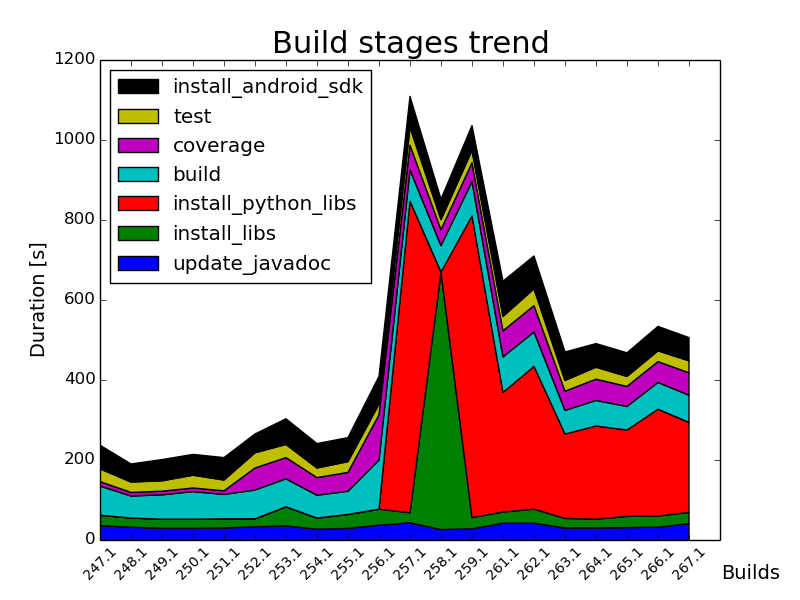
\includegraphics[scale=.45]{pictures/example_matplotlib_trend.png}
  \end{frame}
  \begin{frame}
    \frametitle{Limitations}
    \begin{itemize}
      \item scalability of XML
      \item querying data is limited
      \item developing new charts is not efficient
    \end{itemize}
  \end{frame}
  \begin{frame}
    \frametitle{Integration with Travis CI}
    Call Buildtime Trend scripts in .travis.yml file
    \begin{itemize}
      \item generate timestamps
      \item install dependencies
      \item analyze timestamps and generate chart
      \item store timing data (XML) and chart in gh-pages
    \end{itemize}
  \end{frame}
  \begin{frame}
    \frametitle{Integration with Travis CI}
    This is not ideal!
    \begin{itemize}
      \item scripts become part of the build process
      \item build duration is influenced
      \item complicated to set up
    \end{itemize}
  \end{frame}
  \begin{frame}
    \frametitle{Integration with Travis CI}
    Possible solutions
    \begin{itemize}
      \item create a service that analyses the logfile after the build is finished
      \item store the data in a database outside Travis
      \item host the generated chart(s) outside Travis
    \end{itemize}
    But how?
  \end{frame}
  \begin{frame}
    \frametitle{Keen.io}
    <insert Keen.io logo>
    Keen IO's powerful APIs do the heavy lifting for you, so you can gather all the data you want and start getting the answers you need. 
  \end{frame}
  \begin{frame}
    \frametitle{Keen.io}
    \begin{itemize}
      \item gather data
      \item store it
      \item analyse
      \item visualise
      \item support for several languages, including Python
    \end{itemize}
    Great : this solves the data storage and chart generation problem!
  \end{frame}
  \begin{frame}
    \frametitle{First release - dashboard}
    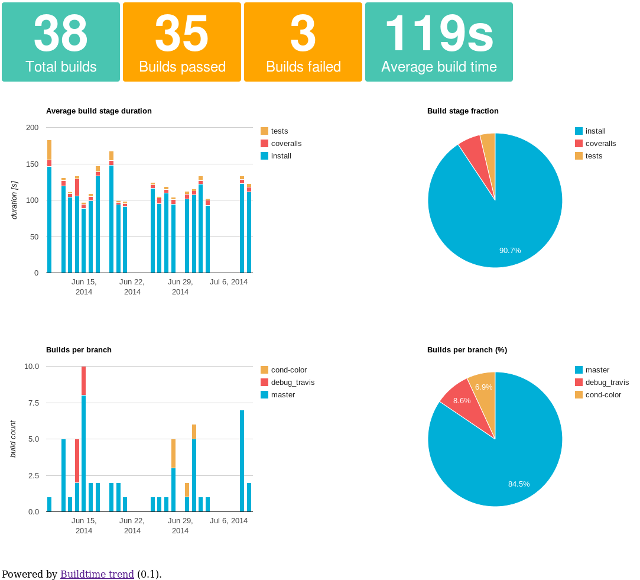
\includegraphics[scale=.45]{pictures/example_dashboard.png}
  \end{frame}
  \begin{frame}
    \frametitle{First release - features}
    \begin{itemize}
      \item scripts tightly coupled with Travis CI build
      \item storing in XML and chart generation with matplotlib (native mode)
      \item storing and chart generation with Keen.io
      \item chart dashboard deployed to gh-pages
    \end{itemize}
    Yeah, it works!\\
    \pause
    But there is still room for improvement.
  \end{frame}
  \begin{frame}
    \frametitle{Travis CI timing data}
    Good news!\\
    Travis CI announces adding timing data to their logs!\\
  \end{frame}
  \begin{frame}
    \frametitle{Create a service}
    \begin{itemize}
      \item get Travis CI build logfile
      \item parse the timing data
      \item store data in Keen.io
    \end{itemize}
  \end{frame}
  \begin{frame}
    \frametitle{Rearrange project structure}
    Create organisation on GitHub to host the different repositories :
    \begin{itemize}
      \item service
      \item client
      \item library (with common functionality)
      \item dashboard
    \end{itemize}
    <Add project schema>
  \end{frame}
  \begin{frame}
    \frametitle{Challenges}
    \begin{itemize}
      \item hosting the service
      \item triggering the service at the end of a build
      \item let the subprojects work together
      \item Open Source license
      \item business model
    \end{itemize}
  \end{frame}
  \begin{frame}
    \frametitle{Hosting the service}
    \begin{itemize}
      \item CherryPy turns scripts into webservice
        \begin{itemize}
          \item dashboard
          \item badge
          \item parse buildlog
        \end{itemize}
      \item service hosted on Heroku : \href{https://buildtimetrend.herokuapp.com/}{https://buildtimetrend.herokuapp.com/}
      \item deploy to Heroku with Travis CI build
    \end{itemize}
  \end{frame}
  \begin{frame}
    \frametitle{Deploy to Heroku during Travis CI build}
    In \textit{.travis.yml} :
    \begin{example}
      \small{deploy:\\
      \ \ provider: heroku\\
      \ \ api\_key:\\
      \ \ \ \ secure: <secure key>\\
      \ \ app:\\
      \ \ \ \ deploy-prod: buildtimetrend}
    \end{example}
    Branch \textit{deploy-prod} is deployed to app \href{https://buildtimetrend.herokuapp.com/}{https://buildtimetrend.herokuapp.com/}
  \end{frame}
  \begin{frame}
    \frametitle{Travis CI triggers service}
    Trigger the service at the end of a Travis CI build in \textit{.travis.yml} :
    \begin{example}
      \small{notifications:\\
      \ \ webhooks:\\
      \ \ \ \ - https://buildtimetrend.herokuapp.com/travis}
    \end{example}
  \end{frame}
  \begin{frame}
    \frametitle{Travis CI triggers service}
    \begin{itemize}
      \item A JSON payload with build data is sent
      \item service identifies repo and build ID
      \item build job data and logfiles are retrieved from Travis CI
      \item build job logfiles are parsed looking for timing tags
      \item build stages duration is calculated
      \item build job data is sent to Keen.io
    \end{itemize}
  \end{frame}
  \begin{frame}
    \frametitle{Demo}
    \begin{itemize}
      \item Service : \href{https://buildtimetrend.herokuapp.com/}{\small{https://buildtimetrend.herokuapp.com/}}
      \item Dashboard : \href{https://buildtimetrend.herokuapp.com/dashboard/buildtimetrend/python-lib/index.html}{\small{https://buildtimetrend.herokuapp.com/dashboard/buildtimetrend/python-lib}}
      \item Badges : \href{https://github.com/buildtimetrend/service\#badge-examples}{\small{https://github.com/buildtimetrend/service\#badge-examples}}
    \end{itemize}
  \end{frame}

  \begin{frame}
    \frametitle{Lessons learned}
    \begin{itemize}
      \item start simple
      \item (re)use as much existing tools as possible
      \item start with what you know, learn new skills as you progress
      \item try, even if it is all scary at first
    \end{itemize}
  \end{frame}
  \begin{frame}
   \frametitle{Questions}
    Thanks for your attention!\\
    Questions?
    \vfill
    Dieter Adriaenssens - \href{https://twitter.com/dcadriaenssens}{@dcadriaenssens}
    \vfill
    Buildtime Trend
    \begin{itemize}
      \item Website : \href{https://buildtimetrend.github.io/}{https://buildtimetrend.github.io/}
      \item Twitter : \href{https://twitter.com/buildtime_trend}{@buildtime\_trend}
    \end{itemize}
  \end{frame}
\end{document}
